\section{Feststellung geeigneter Parameter}
\label{parameters}

Diese Arbeit soll sich im großen Maße mit der Ermittlung geeigneter Parameter für die Einschätzung der Fahrtauglichkeit beschäftigen. Dazu werden im Folgenden verschiedene Parameter aus den im Abschnitt \ref{relatedWork} genannten Richtlinien genannt und erläutert. Im nächsten Schritt werden Möglichkeiten der Messung dieser Parameter aufgeführt. Daraus wird anschließend eine Auswahl von gut messbaren Parametern getroffen, auf welche sich in den folgenden Teilen dieser Arbeit stärker bezogen wird.
\subsection{Ermittlung der Parameter}

Die Richtlinie der Driver \& Vehicle Licensing Agency \cite{drivervehiclelicencingagency} führt bereits ein detaillierten Überblick von zu bewertenden Parametern auf:

\begin{flushleft}
	\begin{multicols}{2}
		\begin{itemize}
			\item Sehvermögen
			\item Visuelle Raumvorstellung
			\item Hörvermögen
			\item Aufmerksamkeit und Konzentration
			\item Gedächtnis
			\item Einsicht und Verständnis
			\item Urteilsfähigkeit
			\item Reaktionsfähigkeit
			\item Persönliche Organisation
			\item Selbstkontrolle
			\item Sensitivität
			\item Körperliche Voraussetzungen
			\item Koordination
			\item Adaptive Strategien (Anpassungsfähigkeit)
		\end{itemize}
	\end{multicols}
\end{flushleft}

Bei den körperlichen Voraussetzung wird hierbei speziell auf die Muskelkraft und - kontrolle verwiesen. Die Begutachtungsleitlinien zur Kraftfahreignung und die daraus abgeleiteten unterstützenden Testverfahren folgen im wesentlichen diesen Parametern, zählen aber die Belastbarkeit und den Stress bzw. Aggression des Fahrers als wichtige Kriterien hinzu \cite{begutachtungsrichtlinien, testverfahrenpsychometrischefahreignung}. Beide Richtlinien beziehen sich vermehrt auf psychische Fahrereigenschaften, zu körperlichen Eigenschaften zählen sie eher Bewegungsbehinderungen und körperliche Erkrankungen. Weitere mögliche Parameter zur Einschätzung der Fahrtauglichkeit können nach Schubert et al. erhöhter Alkohol - bzw. Drogenkonsum, sowie ein Vergleich der Strafakte auf vorhergehende Auffälligkeiten im Straßenverkehr sein  \cite{beurteilungskriterien}. Zumindest zweiteres ist sicherlich datenschutzrechtlich bedenklich.

\subsection{Möglichkeit der Messungen}
Eine Vielzahl der gefundenen Parameter lässt sich sehr gut durch psychologische Tests untersuchen. Diese haben sich in der Praxis bewehrt und könnten auf dem Smartphone eingesetzt werden, indem der Fahrer vor Fahrtantritt eine Reihe solcher Tests absolvieren muss, bevor das Fahrzeug in Bewegung gesetzt werden darf. Poschadel und Falkenstein heben besonders das \textit{Wiener Testsystem} beim Einsatz innerhalb der Verkehrspsychologie hervor \cite{testverfahrenpsychometrischefahreignung}. Dieses wird von der Firma \textit{SCHUHFRIED GmbH} entwickelt und listet insgesamt 113 Einzeltests\footnote{\label{foot:schuhfriedtests} Schuhfried.at. (2018). SCHUHFRIED - Alle Tests. [online] Verfügbar unter: https://www.schuhfried.at/tests/alle-tests/ [Zugriff 28 Jan. 2018].} in verschiedenen Ausführungen zur Überprüfung psychischer Eigenschaften. Beispielsweise sieht man in der Abbildung \ref{fig:atavt} den Adaptiven Tachistoskopischen Verkehrsauffassungstest (ATAVT), der die Anpassungs - und Beobachtungsfähigkeit eines Fahrers im Straßenverkehr testet. Zudem bietet der Entwickler eine Schnittstelleninteraktion der Testsysteme an, um diese in neue Softwaresysteme einzubetten. Somit wäre eine Integration der Tests in mobilen Apps denkbar.

%reset footnote counter, because its set 5 instead of 4 this place
\begingroup
	\newcounter{savefootnote}
	\setcounter{savefootnote}{\value{footnote}}% Store footnote counter
	\setcounter{footnote}{2}% Reset footnote counter
	\renewcommand{\thefootnote}{\alph{footnote}}% Modify footnote printing
\endgroup

\begin{figure}[H]
\centering
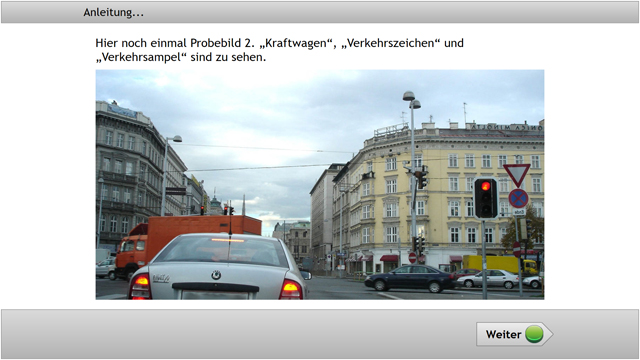
\includegraphics[width=\linewidth]{images/atavt}
\caption[Caption for parameters]{Adaptiver Tachistoskopischer Verkehrsauffassungstest zur Überprüfung der Anpassungs - und Beobachtungsfähigkeit im Straßenverkehr \footnotemark}
\label{fig:atavt}
\end{figure}
\footnotetext{\label{foot:atavt} Schuhfried.at. (2018). SCHUHFRIED - ATAVT. [online] Verfügbar unter: https://www.schuhfried.at/test/ATAVT [Zugriff 1 Feb. 2018].}

Des Weiteren zeigen Studien zum Thema kognitiver Tests in der Verkehrspsychologie, wie unter anderem von Bennett et al. \cite{cognitivetestsfitnesstodrive}, dass oft eine Reihe verschiedener Tests nötig ist, um ein valides Bild der Fahrtauglichkeit zu gewinnen. Über die Qualität einzelner Tests wird im Abschnitt \ref{dataValidity} noch mithilfe von diversen Studien diskutiert. Schwierig wird außerdem das Vorhaben, die genannten Tests auf dem Smartphone in App-Tests abzubilden. Diese Umsetzbarkeit wird nachfolgend im Abschnitt \ref{dataValidity} ebenfalls beurteilt.

Weitere Möglichkeiten der Messung bieten Wearables. Die in ihnen eingebauten Sensoren können Teile der vorher genannten Parameter direkt oder indirekt überprüfen. Tatsächlich hat die Recherche ergeben, dass Wearables bislang selten direkten Einsatz in der Verkehrspsychologie erhalten haben. Zu den Haupteinsatzfeldern gehören zum einen das Messen und Auswerten von Körperfunktionen, wie zum Beispiel die Herzfrequenz. Diese Messfunktionen eignen sich sehr gut, um die körperlichen Voraussetzungen des Fahrers vor Fahrtantritt gezielt auszuwerten. Beispielsweise schätzen Patel et al. die Möglichkeiten von Wearables mit der Messung von Herzfrequenz, Atemfrequenz, Blutdruck, Blutsauerstoffsättigung und Muskelaktivität sehr hoch ein \cite{reviewwearablesensors}. Eine Reihe der in ihrer Arbeit genannten Sensoren sind in gängigen Smartwatches und Fitness-Armbändern jedoch nicht eingebaut. Vielmehr bewerten  El-Amrawy et al. das Potenzial mit der Messung von Fitnessaktivität (über Schrittzähler), Puls, Gewicht, Herzfrequenz, Sauerstoffgehalt im Blut und Schlafmuster etwas geringer \cite{wearabletracking}. Trotzdem lassen sich damit bereits eine Menge von körperlichen Parametern bezüglich der Fahrtauglichkeit einschätzen. Beispielsweise haben Mayya et al. herausgearbeitet, wie man mittels der Herzfrequenzmessung den Stresslevel eines Nutzers bestimmen kann \cite{monitoringstressheartrate}. Choi et al. haben in ihrer Arbeit eine Plattform entwickelt, welche mithilfe von Wearables die Schlafqualität bestimmen kann \cite{platformsleepquality}. Aus diesen Einschätzungen könnte man zum Beispiel die Müdigkeit eines Fahrers bestimmen.  Des Weiteren kann durch eingebaute Gyroskope und andere Sensoren in Wearables die Balance und Koordination eines Fahrers gemessen werden \cite{balancewearables, smartglasses}.  Interessant bleibt zu betrachten, wie präzise und glaubwürdig diese Einschätzung ist. Dies wird im Abschnitt \ref{dataValidity} noch untersucht.

Aus den gewonnen Erkenntnissen der Recherche zu psychologischen und kognitiven Tests zur Fahreignung, sowie aus den erarbeiteten Möglichkeiten zur Ermittlung einzelner Parameter mittels mobilen Sensoren, lässt sich sehr gut eine zweigeteilte Aufteilung der gewählten Parameter erstellen. Dies teilt sich zum einen in die Parameter, die sich mithilfe bewährter psychologischer Tests mittels Smartphone-App überprüfen lassen. Diese werden in der Tabelle \ref{tab:ps} mit zugehöriger Messmethode dargestellt. Das Kürzel dient zur besseren Referenzierung in den folgenden Kapiteln. 

\FloatBarrier
\begin{table}[htbp]
	\caption{Übersicht gewählter Parameter in Messkategorie \textit{App-Tests Smartphone} (PS)}
	\begin{center}
		\resizebox{\linewidth}{!}{
		\begin{tabular}{c c c }
			\hline
			Kürzel& \textbf{Parameter} & \textbf{\textit{Möglichkeit der Messung}}\\
			\hline
			PS01 & Aufmerksamkeit \& Konzentration& Cognitrone-Test (COG)  \\
			PS02 & Sehvermögen& Test nach Albrecht et al. \cite{mobilesmarttracking}, \\
			&& teilweise Linienverfolgungstest (LVT) \\
			PS03 &Visuelle Raumvorstellung&Adaptiver Dreidimensionaler \\
			&&Würfeltest (A3DW), \\ 
			&&Intelligenz-Basis-Funktionen-\\
			&&Test (IBF) \\
			PS04 & Gedächtnis& Visueller Gedächtnistest (VISGED)\\
			PS05 & Belastbarkeit & Wiener Determinationstest (DT) \\
			PS06 & Anpassungsfähigkeit & Adaptiver Tachistoskopischer \\
			&&Verkehrsauffassungstest (ATAVT) \\
			PS07&Reaktionsfähigkeit&Wiener Reaktionstest (RT) \\
			&& Trail-Making-Test (TMT) \\
			PS08&Selbstkontrolle&IVPE-Test \\
			PS09&Persönliche Organisation&Tower of London-Test (TOL-F) \\
			PS10&Alkoholauffälligkeit&Fragebogen zum funktionalen \\
			&&Trinken (FFT), Test \\
			&&nach Albrecht et al. \cite{mobilesmarttracking} \\
			PS11&Aggression&Verkehrsspezifischer Itempool (VIP) \\
			\hline
		\end{tabular}
		}
		\label{tab:ps}
	\end{center}
\end{table}
\FloatBarrier

Die zweite Kategorie umfasst alle die Parameter, die sich mithilfe von Wearables messen lassen. Diese werden in der nachfolgenden Tabelle \ref{tab:pw} dargestellt und erhalten wiederum ein Kürzel zur späteren Referenzierung.

\begin{table}[htbp]
	\caption{Übersicht gewählter Parameter in Messkategorie \textit{Smart-Tracking Wearables} (PW)}
	\begin{center}
		\resizebox{\linewidth}{!}{
		\begin{tabular}{c c c }
			\hline
			Kürzel& \textbf{Parameter} & \textbf{\textit{Möglichkeit der Messung}}\\
			\hline
			PW01 & Körperliche Fitness & Aktivitäts - und  \\
			&& Blutsauerstoffsättigungsmessung \\
			&& (Wearable) \\
			PW02 & Koordination \& Balance & Gyroskop, Accelerometer, \\
			&& Gleichgewichtssensor (Wearable) \\
			&& und Smartglasses \\
			PW03 & Stressliche Belastung & Puls - und \\
			&& Herzfrequenzmessung \\
			&& (Wearable) \\
			PW04 & Müdigkeit & (indirekt) Schlafanalyse \\
			&& (Wearable) \\
			\hline
		\end{tabular}
		}
		\label{tab:pw}
	\end{center}
\end{table}